% Options for packages loaded elsewhere
\PassOptionsToPackage{unicode}{hyperref}
\PassOptionsToPackage{hyphens}{url}
%
\documentclass[
]{article}
\usepackage{lmodern}
\usepackage{amssymb,amsmath}
\usepackage{ifxetex,ifluatex}
\ifnum 0\ifxetex 1\fi\ifluatex 1\fi=0 % if pdftex
  \usepackage[T1]{fontenc}
  \usepackage[utf8]{inputenc}
  \usepackage{textcomp} % provide euro and other symbols
\else % if luatex or xetex
  \usepackage{unicode-math}
  \defaultfontfeatures{Scale=MatchLowercase}
  \defaultfontfeatures[\rmfamily]{Ligatures=TeX,Scale=1}
\fi
% Use upquote if available, for straight quotes in verbatim environments
\IfFileExists{upquote.sty}{\usepackage{upquote}}{}
\IfFileExists{microtype.sty}{% use microtype if available
  \usepackage[]{microtype}
  \UseMicrotypeSet[protrusion]{basicmath} % disable protrusion for tt fonts
}{}
\makeatletter
\@ifundefined{KOMAClassName}{% if non-KOMA class
  \IfFileExists{parskip.sty}{%
    \usepackage{parskip}
  }{% else
    \setlength{\parindent}{0pt}
    \setlength{\parskip}{6pt plus 2pt minus 1pt}}
}{% if KOMA class
  \KOMAoptions{parskip=half}}
\makeatother
\usepackage{xcolor}
\IfFileExists{xurl.sty}{\usepackage{xurl}}{} % add URL line breaks if available
\IfFileExists{bookmark.sty}{\usepackage{bookmark}}{\usepackage{hyperref}}
\hypersetup{
  pdftitle={Chapter 6 in ISLR: Part 1 Model Selection},
  pdfauthor={Laura Kapitula},
  hidelinks,
  pdfcreator={LaTeX via pandoc}}
\urlstyle{same} % disable monospaced font for URLs
\usepackage[margin=1in]{geometry}
\usepackage{color}
\usepackage{fancyvrb}
\newcommand{\VerbBar}{|}
\newcommand{\VERB}{\Verb[commandchars=\\\{\}]}
\DefineVerbatimEnvironment{Highlighting}{Verbatim}{commandchars=\\\{\}}
% Add ',fontsize=\small' for more characters per line
\usepackage{framed}
\definecolor{shadecolor}{RGB}{248,248,248}
\newenvironment{Shaded}{\begin{snugshade}}{\end{snugshade}}
\newcommand{\AlertTok}[1]{\textcolor[rgb]{0.94,0.16,0.16}{#1}}
\newcommand{\AnnotationTok}[1]{\textcolor[rgb]{0.56,0.35,0.01}{\textbf{\textit{#1}}}}
\newcommand{\AttributeTok}[1]{\textcolor[rgb]{0.77,0.63,0.00}{#1}}
\newcommand{\BaseNTok}[1]{\textcolor[rgb]{0.00,0.00,0.81}{#1}}
\newcommand{\BuiltInTok}[1]{#1}
\newcommand{\CharTok}[1]{\textcolor[rgb]{0.31,0.60,0.02}{#1}}
\newcommand{\CommentTok}[1]{\textcolor[rgb]{0.56,0.35,0.01}{\textit{#1}}}
\newcommand{\CommentVarTok}[1]{\textcolor[rgb]{0.56,0.35,0.01}{\textbf{\textit{#1}}}}
\newcommand{\ConstantTok}[1]{\textcolor[rgb]{0.00,0.00,0.00}{#1}}
\newcommand{\ControlFlowTok}[1]{\textcolor[rgb]{0.13,0.29,0.53}{\textbf{#1}}}
\newcommand{\DataTypeTok}[1]{\textcolor[rgb]{0.13,0.29,0.53}{#1}}
\newcommand{\DecValTok}[1]{\textcolor[rgb]{0.00,0.00,0.81}{#1}}
\newcommand{\DocumentationTok}[1]{\textcolor[rgb]{0.56,0.35,0.01}{\textbf{\textit{#1}}}}
\newcommand{\ErrorTok}[1]{\textcolor[rgb]{0.64,0.00,0.00}{\textbf{#1}}}
\newcommand{\ExtensionTok}[1]{#1}
\newcommand{\FloatTok}[1]{\textcolor[rgb]{0.00,0.00,0.81}{#1}}
\newcommand{\FunctionTok}[1]{\textcolor[rgb]{0.00,0.00,0.00}{#1}}
\newcommand{\ImportTok}[1]{#1}
\newcommand{\InformationTok}[1]{\textcolor[rgb]{0.56,0.35,0.01}{\textbf{\textit{#1}}}}
\newcommand{\KeywordTok}[1]{\textcolor[rgb]{0.13,0.29,0.53}{\textbf{#1}}}
\newcommand{\NormalTok}[1]{#1}
\newcommand{\OperatorTok}[1]{\textcolor[rgb]{0.81,0.36,0.00}{\textbf{#1}}}
\newcommand{\OtherTok}[1]{\textcolor[rgb]{0.56,0.35,0.01}{#1}}
\newcommand{\PreprocessorTok}[1]{\textcolor[rgb]{0.56,0.35,0.01}{\textit{#1}}}
\newcommand{\RegionMarkerTok}[1]{#1}
\newcommand{\SpecialCharTok}[1]{\textcolor[rgb]{0.00,0.00,0.00}{#1}}
\newcommand{\SpecialStringTok}[1]{\textcolor[rgb]{0.31,0.60,0.02}{#1}}
\newcommand{\StringTok}[1]{\textcolor[rgb]{0.31,0.60,0.02}{#1}}
\newcommand{\VariableTok}[1]{\textcolor[rgb]{0.00,0.00,0.00}{#1}}
\newcommand{\VerbatimStringTok}[1]{\textcolor[rgb]{0.31,0.60,0.02}{#1}}
\newcommand{\WarningTok}[1]{\textcolor[rgb]{0.56,0.35,0.01}{\textbf{\textit{#1}}}}
\usepackage{graphicx,grffile}
\makeatletter
\def\maxwidth{\ifdim\Gin@nat@width>\linewidth\linewidth\else\Gin@nat@width\fi}
\def\maxheight{\ifdim\Gin@nat@height>\textheight\textheight\else\Gin@nat@height\fi}
\makeatother
% Scale images if necessary, so that they will not overflow the page
% margins by default, and it is still possible to overwrite the defaults
% using explicit options in \includegraphics[width, height, ...]{}
\setkeys{Gin}{width=\maxwidth,height=\maxheight,keepaspectratio}
% Set default figure placement to htbp
\makeatletter
\def\fps@figure{htbp}
\makeatother
\setlength{\emergencystretch}{3em} % prevent overfull lines
\providecommand{\tightlist}{%
  \setlength{\itemsep}{0pt}\setlength{\parskip}{0pt}}
\setcounter{secnumdepth}{-\maxdimen} % remove section numbering

\title{Chapter 6 in ISLR: Part 1 Model Selection}
\author{Laura Kapitula}
\date{11/4/2020}

\begin{document}
\maketitle

\begin{Shaded}
\begin{Highlighting}[]
\KeywordTok{library}\NormalTok{(ISLR) }\CommentTok{#contains the credit data}
\KeywordTok{library}\NormalTok{(tidyverse)}
\KeywordTok{library}\NormalTok{(moderndive)}
\KeywordTok{library}\NormalTok{(skimr)}
\KeywordTok{theme_set}\NormalTok{(}\KeywordTok{theme_classic}\NormalTok{())}
\end{Highlighting}
\end{Shaded}

some of the data analysis below is adapted from
\url{http://www.science.smith.edu/~jcrouser/SDS293/labs/lab8-r.html}
\#\# Model Selection and Shrinkage

Recall the linear model
\[Y=\beta_0 + \beta_1X_1+ \beta_2X_2 + \beta_pX_p \]

\begin{itemize}
\tightlist
\item
  How can we find a sweet spot in the variance bias trade-off?
\item
  We consider some approaches for model selection and regularization (ie
  shrinkage).
\end{itemize}

\hypertarget{three-classes-of-methods}{%
\subsection{Three classes of methods}\label{three-classes-of-methods}}

\begin{itemize}
\tightlist
\item
  \textbf{Subset Selection}. We identify a subset of the p predictors
  that we believe to be related to the response. We then fit a model
  using least squares on the reduced set of variables.
\item
  \textbf{Shrinkage}. We fit a model involving all p predictors, but the
  estimated coefficients are shrunken towards zero relative to the least
  squares estimates. This shrinkage (also known as regularization) has
  the effect of reducing variance and can also perform variable
  selection.
\item
  \textbf{Dimension Reduction}. This is also sometimes called automatic
  feature creation. We project the p predictors into a M-dimensional
  subspace, where M \textless{} p.~This is achieved by computing M
  different linear combinations, or projections, of the variables. Then
  these M projections are used as predictors to fit a linear regression
  model by least squares.
\end{itemize}

\hypertarget{subset-selection}{%
\subsection{Subset Selection}\label{subset-selection}}

\emph{Best subset and stepwise model selection procedures}

\hypertarget{best-subset-selection}{%
\subsection{Best Subset Selection}\label{best-subset-selection}}

\begin{enumerate}
\def\labelenumi{\arabic{enumi}.}
\tightlist
\item
  Let \(M_o\) denote the null model, which contains no predictors. This
  model simply predicts the sample mean for each observation.
\item
  For \(k = 1, 2, ...,p\):
\end{enumerate}

\begin{enumerate}
\def\labelenumi{\alph{enumi}.}
\tightlist
\item
  Fit all \({p \choose k} = p!/\left[k!(p-k)!\right]\) combinations of
  models that contain exactly models that contain exactly k predictors.
\item
  Pick the best among these models and call it \(M_k\). Here best can be
  defined as having the smallest \(RSS\), or equivalently largest
  \(R^2\).
\end{enumerate}

\begin{enumerate}
\def\labelenumi{\arabic{enumi}.}
\setcounter{enumi}{2}
\tightlist
\item
  Select a single best model from among \(M_0,...,M_p\) using
  cross-validated prediction error, \(C_p\)(AIC), BIC, or adjusted
  \(R^2\).
\end{enumerate}

\hypertarget{example--credit-data-set}{%
\subsection{Example- Credit data set}\label{example--credit-data-set}}

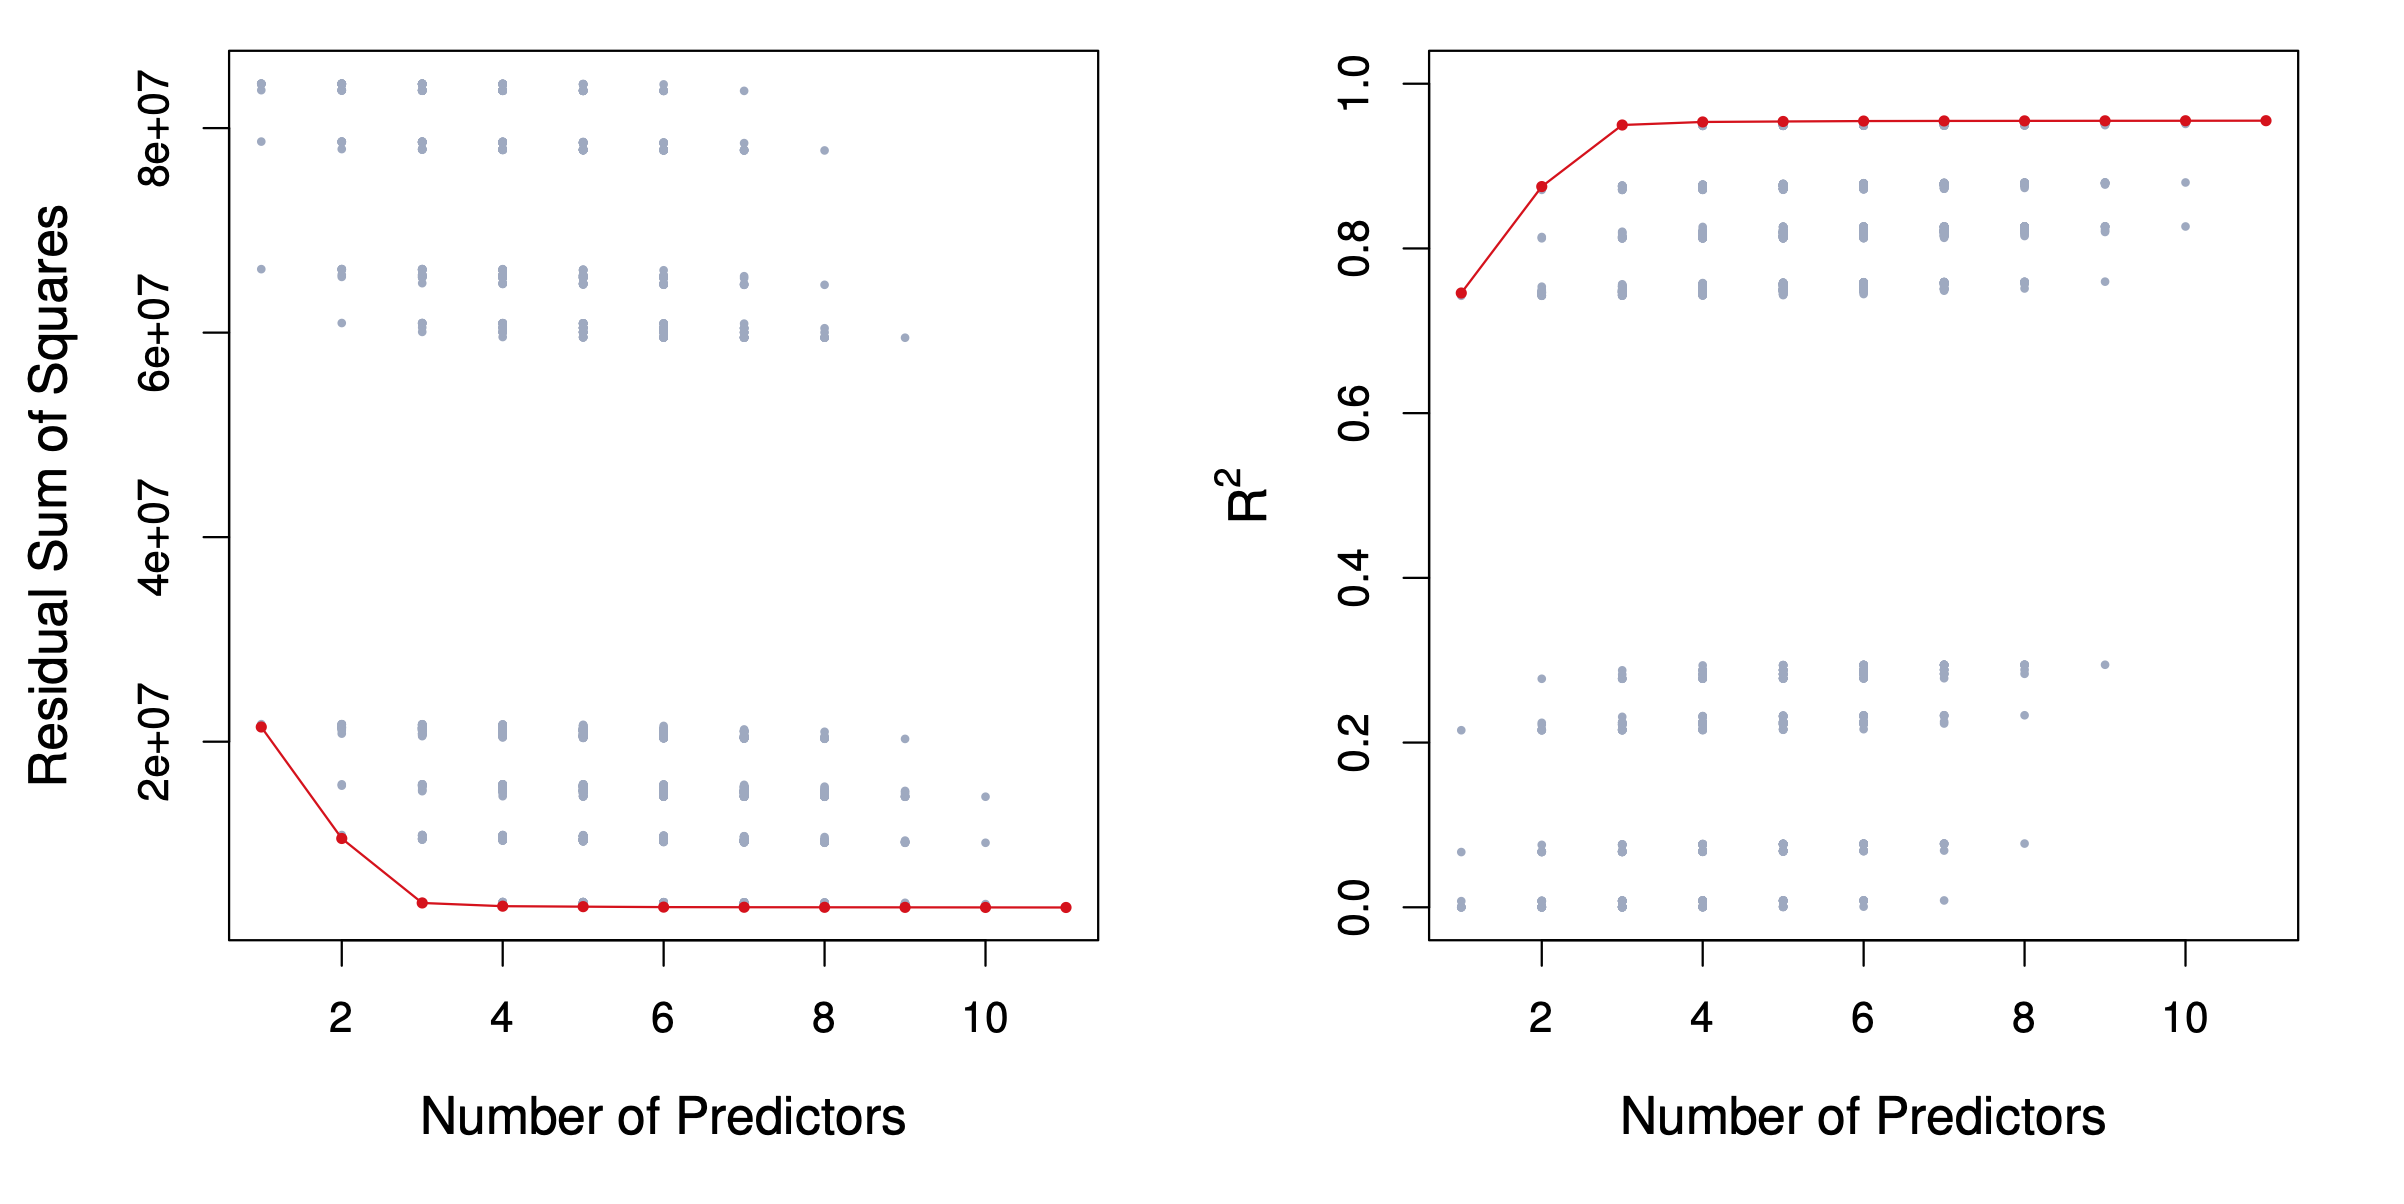
\includegraphics[width=33.39in]{images/6.1} For each possible model
containing a subset of the ten predictors in the Credit data set, the
RSS and \(R^2\) are displayed. The red frontier tracks the best model
for a given number of predictors, according to RSS and \(R^2\). Though
the data set contains only ten predictors, the x-axis ranges from 1 to
11, since one of the variables is categorical and takes on three values,
leading to the creation of two dummy variables

Best subset with \texttt{regsubsets}

\begin{Shaded}
\begin{Highlighting}[]
\KeywordTok{data}\NormalTok{(Credit, }\DataTypeTok{package =} \StringTok{"ISLR"}\NormalTok{)}
\KeywordTok{library}\NormalTok{(leaps) }\CommentTok{# where regsubsets is found}
\NormalTok{regfit_full=}\StringTok{ }\KeywordTok{regsubsets}\NormalTok{(Balance }\OperatorTok{~}\StringTok{ }\NormalTok{., }\DataTypeTok{data=}\NormalTok{Credit[}\DecValTok{2}\OperatorTok{:}\DecValTok{12}\NormalTok{]) }\CommentTok{#id is in column 1, so I leave it off}
\NormalTok{reg_summary=}\KeywordTok{summary}\NormalTok{(regfit_full)}
\NormalTok{reg_summary}
\end{Highlighting}
\end{Shaded}

\begin{verbatim}
## Subset selection object
## Call: regsubsets.formula(Balance ~ ., data = Credit[2:12])
## 11 Variables  (and intercept)
##                    Forced in Forced out
## Income                 FALSE      FALSE
## Limit                  FALSE      FALSE
## Rating                 FALSE      FALSE
## Cards                  FALSE      FALSE
## Age                    FALSE      FALSE
## Education              FALSE      FALSE
## GenderFemale           FALSE      FALSE
## StudentYes             FALSE      FALSE
## MarriedYes             FALSE      FALSE
## EthnicityAsian         FALSE      FALSE
## EthnicityCaucasian     FALSE      FALSE
## 1 subsets of each size up to 8
## Selection Algorithm: exhaustive
##          Income Limit Rating Cards Age Education GenderFemale StudentYes
## 1  ( 1 ) " "    " "   "*"    " "   " " " "       " "          " "       
## 2  ( 1 ) "*"    " "   "*"    " "   " " " "       " "          " "       
## 3  ( 1 ) "*"    " "   "*"    " "   " " " "       " "          "*"       
## 4  ( 1 ) "*"    "*"   " "    "*"   " " " "       " "          "*"       
## 5  ( 1 ) "*"    "*"   "*"    "*"   " " " "       " "          "*"       
## 6  ( 1 ) "*"    "*"   "*"    "*"   "*" " "       " "          "*"       
## 7  ( 1 ) "*"    "*"   "*"    "*"   "*" " "       "*"          "*"       
## 8  ( 1 ) "*"    "*"   "*"    "*"   "*" " "       "*"          "*"       
##          MarriedYes EthnicityAsian EthnicityCaucasian
## 1  ( 1 ) " "        " "            " "               
## 2  ( 1 ) " "        " "            " "               
## 3  ( 1 ) " "        " "            " "               
## 4  ( 1 ) " "        " "            " "               
## 5  ( 1 ) " "        " "            " "               
## 6  ( 1 ) " "        " "            " "               
## 7  ( 1 ) " "        " "            " "               
## 8  ( 1 ) " "        "*"            " "
\end{verbatim}

Best model with 4 variables includes: Income, Limit, Cards, Student.

\hypertarget{choosing-k}{%
\subsection{Choosing k}\label{choosing-k}}

Naturally, RSS and \(R^2=1−RSS/TSS\) improve as we increase k.

To optimize k, we want to minimize the test error, not the training
error.

We could use cross-validation, or alternative estimates of test error:

\begin{itemize}
\tightlist
\item
  Akaike Information Criterion (AIC) (closely related to Mallow's
  \(C_p\)) given an estimate of the irreducible error \(\hat{\sigma^2}\)
  : \[\frac{1}{n}(\text{RSS}+2k\hat\sigma^2)\]
\item
  Bayesian Information Criterion (BIC):
\end{itemize}

\[\frac{1}{n}(\text{RSS}+\log(n)k\hat\sigma^2)\] * Adjusted R2:

\[R^2_a = 1-\frac{\text{RSS}/(n-k-1)}{\text{TSS}/(n-1)}\] Notice that
rather than letting the results of our call to the \texttt{summary()}
function print to the screen, we've saved the results to a variable
called \texttt{reg\_summary}. That way, we can access just the parts we
need. Let's see what's in there:

\begin{Shaded}
\begin{Highlighting}[]
\KeywordTok{names}\NormalTok{(reg_summary)}
\end{Highlighting}
\end{Shaded}

\begin{verbatim}
## [1] "which"  "rsq"    "rss"    "adjr2"  "cp"     "bic"    "outmat" "obj"
\end{verbatim}

Excellent! In addition to the verbose output we get when we print the
summary to the screen, the \texttt{summary()} function also returns
\(R^2 (\tt{rsq})\), RSS, adjusted \(R^2\), \(C_p\), and BIC. We can
examine these to try to select the best overall model. Let's start by
looking at \(R^2\):

\begin{Shaded}
\begin{Highlighting}[]
\NormalTok{reg_summary}\OperatorTok{$}\NormalTok{rsq}
\end{Highlighting}
\end{Shaded}

\begin{verbatim}
## [1] 0.7458484 0.8751179 0.9498788 0.9535800 0.9541606 0.9546879 0.9548167
## [8] 0.9548880
\end{verbatim}

We see that the \(R^2\) statistic increases from 75\% when only one
variable is included in the model to over 95\% when all variables are
included. As expected, the \(R^2\) statistic increases monotonically as
more variables are included.

Plotting RSS, adjusted \(R^2\), \(C_p\), and BIC for all of the models
at once will help us decide which model to select. Note the
\texttt{type="l"} option tells \texttt{R} to connect the plotted points
with lines:

\begin{Shaded}
\begin{Highlighting}[]
\CommentTok{# code below from http://www.science.smith.edu/~jcrouser/SDS293/labs/lab8-r.html}
\CommentTok{# Set up a 2x2 grid so we can look at 4 plots at once}
\KeywordTok{par}\NormalTok{(}\DataTypeTok{mfrow =} \KeywordTok{c}\NormalTok{(}\DecValTok{2}\NormalTok{,}\DecValTok{2}\NormalTok{))}
\KeywordTok{plot}\NormalTok{(reg_summary}\OperatorTok{$}\NormalTok{rss, }\DataTypeTok{xlab =} \StringTok{"Number of Variables"}\NormalTok{, }\DataTypeTok{ylab =} \StringTok{"RSS"}\NormalTok{, }\DataTypeTok{type =} \StringTok{"l"}\NormalTok{)}
\KeywordTok{plot}\NormalTok{(reg_summary}\OperatorTok{$}\NormalTok{adjr2, }\DataTypeTok{xlab =} \StringTok{"Number of Variables"}\NormalTok{, }\DataTypeTok{ylab =} \StringTok{"Adjusted RSq"}\NormalTok{, }\DataTypeTok{type =} \StringTok{"l"}\NormalTok{)}

\CommentTok{# We will now plot a red dot to indicate the model with the largest adjusted R^2 statistic.}
\CommentTok{# The which.max() function can be used to identify the location of the maximum point of a vector}
\NormalTok{adj_r2_max =}\StringTok{ }\KeywordTok{which.max}\NormalTok{(reg_summary}\OperatorTok{$}\NormalTok{adjr2) }
\CommentTok{# The points() command works like the plot() command, except that it puts points }
\CommentTok{# on a plot that has already been created instead of creating a new plot}
\KeywordTok{points}\NormalTok{(adj_r2_max, reg_summary}\OperatorTok{$}\NormalTok{adjr2[adj_r2_max], }\DataTypeTok{col =}\StringTok{"red"}\NormalTok{, }\DataTypeTok{cex =} \DecValTok{2}\NormalTok{, }\DataTypeTok{pch =} \DecValTok{20}\NormalTok{)}

\CommentTok{# We'll do the same for C_p and BIC, this time looking for the models with the SMALLEST statistic}
\KeywordTok{plot}\NormalTok{(reg_summary}\OperatorTok{$}\NormalTok{cp, }\DataTypeTok{xlab =} \StringTok{"Number of Variables"}\NormalTok{, }\DataTypeTok{ylab =} \StringTok{"Cp"}\NormalTok{, }\DataTypeTok{type =} \StringTok{"l"}\NormalTok{)}
\NormalTok{cp_min =}\StringTok{ }\KeywordTok{which.min}\NormalTok{(reg_summary}\OperatorTok{$}\NormalTok{cp) }
\KeywordTok{points}\NormalTok{(cp_min, reg_summary}\OperatorTok{$}\NormalTok{cp[cp_min], }\DataTypeTok{col =} \StringTok{"red"}\NormalTok{, }\DataTypeTok{cex =} \DecValTok{2}\NormalTok{, }\DataTypeTok{pch =} \DecValTok{20}\NormalTok{)}

\KeywordTok{plot}\NormalTok{(reg_summary}\OperatorTok{$}\NormalTok{bic, }\DataTypeTok{xlab =} \StringTok{"Number of Variables"}\NormalTok{, }\DataTypeTok{ylab =} \StringTok{"BIC"}\NormalTok{, }\DataTypeTok{type =} \StringTok{"l"}\NormalTok{)}
\NormalTok{bic_min =}\StringTok{ }\KeywordTok{which.min}\NormalTok{(reg_summary}\OperatorTok{$}\NormalTok{bic) }
\KeywordTok{points}\NormalTok{(bic_min, reg_summary}\OperatorTok{$}\NormalTok{bic[bic_min], }\DataTypeTok{col =} \StringTok{"red"}\NormalTok{, }\DataTypeTok{cex =} \DecValTok{2}\NormalTok{, }\DataTypeTok{pch =} \DecValTok{20}\NormalTok{)}
\end{Highlighting}
\end{Shaded}

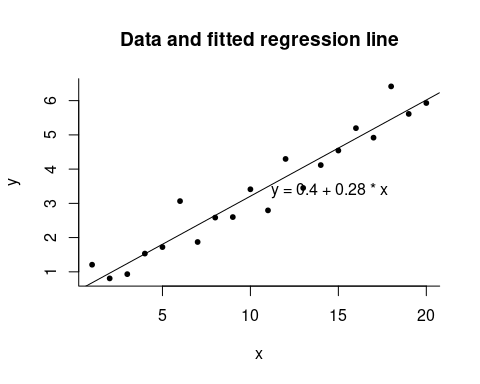
\includegraphics{ISLR_chapter6_selection_files/figure-latex/unnamed-chunk-5-1.pdf}
Recall that in the second step of our selection process, we narrowed the
field down to just one model on any \(k<=p\) predictors. We see that
according to BIC, the best performer is the model with 4 variables.
According to \(C_p\), 6 variables. Adjusted \(R^2\) suggests that 7
might be best. No one measure and no one model will necessarily be
flagged as best.

The \texttt{regsubsets()} function has a built-in \texttt{plot()}
command which can be used to display the selected variables for the best
model with a given number of predictors, ranked according to a chosen
statistic. The top row of each plot contains a black square for each
variable selected according to the optimal model associated with that
statistic.

To find out more about this function, type \texttt{?plot.regsubsets}.

\begin{Shaded}
\begin{Highlighting}[]
\KeywordTok{plot}\NormalTok{(regfit_full, }\DataTypeTok{scale=}\StringTok{"r2"}\NormalTok{)}
\end{Highlighting}
\end{Shaded}

\includegraphics{ISLR_chapter6_selection_files/figure-latex/unnamed-chunk-6-1.pdf}

As expected, \(R^2\) is maximized by the model that contains all the
predictors.

\begin{Shaded}
\begin{Highlighting}[]
\KeywordTok{plot}\NormalTok{(regfit_full, }\DataTypeTok{scale=}\StringTok{"adjr2"}\NormalTok{)}
\end{Highlighting}
\end{Shaded}

\includegraphics{ISLR_chapter6_selection_files/figure-latex/unnamed-chunk-7-1.pdf}

Adjusted \(R^2\) downselects to 7 predictors. We can use the
\texttt{coef()} function to see which predictors made the cut:

\begin{Shaded}
\begin{Highlighting}[]
\KeywordTok{coef}\NormalTok{(regfit_full, }\DecValTok{7}\NormalTok{)}
\end{Highlighting}
\end{Shaded}

\begin{verbatim}
##  (Intercept)       Income        Limit       Rating        Cards          Age 
## -488.6158695   -7.8036338    0.1936237    1.0940490   18.1091708   -0.6206538 
## GenderFemale   StudentYes 
##  -10.4531521  426.5812620
\end{verbatim}

\begin{Shaded}
\begin{Highlighting}[]
\KeywordTok{plot}\NormalTok{(regfit_full, }\DataTypeTok{scale=}\StringTok{"Cp"}\NormalTok{)}
\end{Highlighting}
\end{Shaded}

\includegraphics{ISLR_chapter6_selection_files/figure-latex/unnamed-chunk-9-1.pdf}

\(C_p\) downselects further to 6 variables.

\begin{Shaded}
\begin{Highlighting}[]
\KeywordTok{coef}\NormalTok{(regfit_full, }\DecValTok{6}\NormalTok{)}
\end{Highlighting}
\end{Shaded}

\begin{verbatim}
##  (Intercept)       Income        Limit       Rating        Cards          Age 
## -493.7341870   -7.7950824    0.1936914    1.0911874   18.2118976   -0.6240560 
##   StudentYes 
##  425.6099369
\end{verbatim}

\begin{Shaded}
\begin{Highlighting}[]
\KeywordTok{plot}\NormalTok{(regfit_full, }\DataTypeTok{scale=}\StringTok{"bic"}\NormalTok{)}
\end{Highlighting}
\end{Shaded}

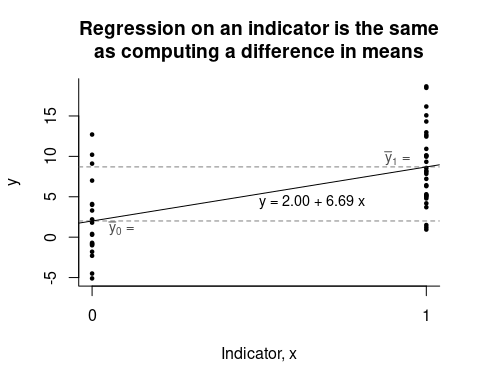
\includegraphics{ISLR_chapter6_selection_files/figure-latex/unnamed-chunk-11-1.pdf}

We see that several models share a BIC close to -1200. However, the
model with the lowest BIC is the four-variable model given below.

\begin{Shaded}
\begin{Highlighting}[]
\KeywordTok{coef}\NormalTok{(regfit_full, }\DecValTok{4}\NormalTok{)}
\end{Highlighting}
\end{Shaded}

\begin{verbatim}
##  (Intercept)       Income        Limit        Cards   StudentYes 
## -499.7272117   -7.8392288    0.2666445   23.1753794  429.6064203
\end{verbatim}

\hypertarget{forward-and-backward-stepwise-selection}{%
\section{Forward and Backward Stepwise
Selection}\label{forward-and-backward-stepwise-selection}}

For computational reasons, best subset selection cannot be applied with
very large p.~Why not?

\begin{itemize}
\tightlist
\item
  Best subset selection may also suffer from statistical problems when p
  is large: larger the search space, the higher the chance of finding
  models that look good on the training data, even though they might not
  have any predictive power on future data.
\item
  Thus an enormous search space can lead to overfitting and high
  variance of the coefficient estimates.
\item
  For both of these reasons, stepwise methods, which explore a far more
  restricted set of models, are attractive alternatives to best subset
  selection.
\end{itemize}

There are simulations that have been done that have shown Stepwise
methods will often not work well at finding important predictive
variables so do remember just because a stepwise method drops or brings
in a variable it does NOT mean that variable is necessarily important or
not-important. If your only goal is prediction and you use
cross-validation to evaluate the models suggested by stepwise methods
they can be used to find a decent predictive model, but I would
recommend using a shrinkage method over stepwise. I would NEVER
recommend using stepwise using p-value for model selection. Remember
once you do model selection your p-values are basically meaningless
because all the theory assumes you know the correct model before you
start.

\hypertarget{forward-stepwise-selection}{%
\subsection{Forward Stepwise
Selection}\label{forward-stepwise-selection}}

\begin{itemize}
\item
  Forward stepwise selection begins with a model containing no
  predictors, and then adds predictors to the model, one-at-a-time,
  until all of the predictors are in the model.
\item
  In particular, at each step the variable that gives the greatest
  \emph{additional} improvement to the fit is added to the model.
\item
  In Detail
\end{itemize}

\begin{enumerate}
\def\labelenumi{\arabic{enumi}.}
\tightlist
\item
  Let \(M_o\) denote the null model, which contains no predictors. This
  model simply predicts the sample mean for each observation.
\item
  For \(k = 0,1, 2, ...,p-1\):
\end{enumerate}

\begin{enumerate}
\def\labelenumi{\alph{enumi}.}
\tightlist
\item
  Consider all all \(p - k\) models that augment the predictors in
  \(M_k\) with one additional predictor.\\
\item
  Choose the \emph{best} among these \(p-k\) models and call it
  \(M_{k+1}\). Here \emph{best} is defined as having the smallest
  \(RSS\), or equivalently largest \(R^2\).
\end{enumerate}

\begin{enumerate}
\def\labelenumi{\arabic{enumi}.}
\setcounter{enumi}{2}
\tightlist
\item
  Select a single best model from among \(M_0,...,M_p\) using
  cross-validated prediction error, \(C_p\)(AIC), BIC, or adjusted
  \(R^2\).
\end{enumerate}

That forward stepwise selection has a computational advantage over best
subset selection is clear. However, it is not guaranteed to find the
best possible model out of all \(2^p\) models ubsets of the p
predictors.

We can also use the \texttt{regsubsets()} function to perform forward
stepwise or backward stepwise selection, using the argument
\texttt{method="forward"} or \texttt{method="backward"}.

\begin{Shaded}
\begin{Highlighting}[]
\CommentTok{# Forward}
\NormalTok{regfit_fwd =}\StringTok{ }\KeywordTok{regsubsets}\NormalTok{(Balance }\OperatorTok{~}\StringTok{ }\NormalTok{., }\DataTypeTok{data=}\NormalTok{Credit[}\DecValTok{2}\OperatorTok{:}\DecValTok{12}\NormalTok{], }\DataTypeTok{nvmax=}\DecValTok{11}\NormalTok{, }\DataTypeTok{method=}\StringTok{"forward"}\NormalTok{)}
\KeywordTok{summary}\NormalTok{(regfit_fwd)}
\end{Highlighting}
\end{Shaded}

\begin{verbatim}
## Subset selection object
## Call: regsubsets.formula(Balance ~ ., data = Credit[2:12], nvmax = 11, 
##     method = "forward")
## 11 Variables  (and intercept)
##                    Forced in Forced out
## Income                 FALSE      FALSE
## Limit                  FALSE      FALSE
## Rating                 FALSE      FALSE
## Cards                  FALSE      FALSE
## Age                    FALSE      FALSE
## Education              FALSE      FALSE
## GenderFemale           FALSE      FALSE
## StudentYes             FALSE      FALSE
## MarriedYes             FALSE      FALSE
## EthnicityAsian         FALSE      FALSE
## EthnicityCaucasian     FALSE      FALSE
## 1 subsets of each size up to 11
## Selection Algorithm: forward
##           Income Limit Rating Cards Age Education GenderFemale StudentYes
## 1  ( 1 )  " "    " "   "*"    " "   " " " "       " "          " "       
## 2  ( 1 )  "*"    " "   "*"    " "   " " " "       " "          " "       
## 3  ( 1 )  "*"    " "   "*"    " "   " " " "       " "          "*"       
## 4  ( 1 )  "*"    "*"   "*"    " "   " " " "       " "          "*"       
## 5  ( 1 )  "*"    "*"   "*"    "*"   " " " "       " "          "*"       
## 6  ( 1 )  "*"    "*"   "*"    "*"   "*" " "       " "          "*"       
## 7  ( 1 )  "*"    "*"   "*"    "*"   "*" " "       "*"          "*"       
## 8  ( 1 )  "*"    "*"   "*"    "*"   "*" " "       "*"          "*"       
## 9  ( 1 )  "*"    "*"   "*"    "*"   "*" " "       "*"          "*"       
## 10  ( 1 ) "*"    "*"   "*"    "*"   "*" " "       "*"          "*"       
## 11  ( 1 ) "*"    "*"   "*"    "*"   "*" "*"       "*"          "*"       
##           MarriedYes EthnicityAsian EthnicityCaucasian
## 1  ( 1 )  " "        " "            " "               
## 2  ( 1 )  " "        " "            " "               
## 3  ( 1 )  " "        " "            " "               
## 4  ( 1 )  " "        " "            " "               
## 5  ( 1 )  " "        " "            " "               
## 6  ( 1 )  " "        " "            " "               
## 7  ( 1 )  " "        " "            " "               
## 8  ( 1 )  " "        "*"            " "               
## 9  ( 1 )  "*"        "*"            " "               
## 10  ( 1 ) "*"        "*"            "*"               
## 11  ( 1 ) "*"        "*"            "*"
\end{verbatim}

Compare the models with 1-4 predictors here to what we got for best
subsets. What do you notice? First three are the same, but 4 predictor
model is different.

\hypertarget{backward-stepwise-selection}{%
\subsection{Backward Stepwise
Selection}\label{backward-stepwise-selection}}

\begin{itemize}
\item
  Like forward stepwise selection, backward stepwise selection provides
  an efficient alternative to best subset selection.
\item
  However, unlike forward stepwise selection, it begins with the full
  least squares model containing all p predictors, and then iteratively
  removes the least useful predictor, one-at-a-time.
\item
  In Detail
\end{itemize}

\begin{enumerate}
\def\labelenumi{\arabic{enumi}.}
\tightlist
\item
  Let \(M_p\) denote the full model, which contains all the predictors.
\item
  For \$k =p, p-1, \ldots, 1 \$:
\end{enumerate}

\begin{enumerate}
\def\labelenumi{\alph{enumi}.}
\tightlist
\item
  Consider all all \(k\) models that contain all but one of the
  predictors in \(M_k\) for a total of \(k-1\) predictors.
\item
  Choose the \emph{best} among these \(k\) models and call it
  \(M_{k-1}\). Here \emph{best} is defined as having the smallest
  \(RSS\), or equivalently largest \(R^2\).
\end{enumerate}

\begin{enumerate}
\def\labelenumi{\arabic{enumi}.}
\setcounter{enumi}{2}
\tightlist
\item
  Select a single best model from among \(M_0,...,M_p\) using
  cross-validated prediction error, \(C_p\)(AIC), BIC, or adjusted
  \(R^2\).
\end{enumerate}

\begin{itemize}
\tightlist
\item
  Like forward stepwise selection, the backward selection approach
  searches through only \(1 + p(p + 1)/2\) models, and so can be applied
  in settings where p is too large to apply best subset selection
\item
  Like forward stepwise selection, backward stepwise selection is not
  guaranteed to yield the \emph{best} model containing a subset of the
  \(p\) predictors.
\item
  Backward selection requires that the \emph{number of samples n is
  larger than the number of variables p} (so that the full model can be
  fit). In contrast, forward stepwise can be used even when \(n < p\),
  and so is the only viable subset method when \(p\) is very large.
\end{itemize}

For the \texttt{Credit} data.

\begin{Shaded}
\begin{Highlighting}[]
\CommentTok{# Backward}
\NormalTok{regfit_bwd =}\StringTok{ }\KeywordTok{regsubsets}\NormalTok{(Balance }\OperatorTok{~}\StringTok{ }\NormalTok{., }\DataTypeTok{data=}\NormalTok{Credit[}\DecValTok{2}\OperatorTok{:}\DecValTok{12}\NormalTok{], }\DataTypeTok{nvmax=}\DecValTok{11}\NormalTok{, }\DataTypeTok{method=}\StringTok{"backward"}\NormalTok{)}
\KeywordTok{summary}\NormalTok{(regfit_bwd)}
\end{Highlighting}
\end{Shaded}

\begin{verbatim}
## Subset selection object
## Call: regsubsets.formula(Balance ~ ., data = Credit[2:12], nvmax = 11, 
##     method = "backward")
## 11 Variables  (and intercept)
##                    Forced in Forced out
## Income                 FALSE      FALSE
## Limit                  FALSE      FALSE
## Rating                 FALSE      FALSE
## Cards                  FALSE      FALSE
## Age                    FALSE      FALSE
## Education              FALSE      FALSE
## GenderFemale           FALSE      FALSE
## StudentYes             FALSE      FALSE
## MarriedYes             FALSE      FALSE
## EthnicityAsian         FALSE      FALSE
## EthnicityCaucasian     FALSE      FALSE
## 1 subsets of each size up to 11
## Selection Algorithm: backward
##           Income Limit Rating Cards Age Education GenderFemale StudentYes
## 1  ( 1 )  " "    "*"   " "    " "   " " " "       " "          " "       
## 2  ( 1 )  "*"    "*"   " "    " "   " " " "       " "          " "       
## 3  ( 1 )  "*"    "*"   " "    " "   " " " "       " "          "*"       
## 4  ( 1 )  "*"    "*"   " "    "*"   " " " "       " "          "*"       
## 5  ( 1 )  "*"    "*"   "*"    "*"   " " " "       " "          "*"       
## 6  ( 1 )  "*"    "*"   "*"    "*"   "*" " "       " "          "*"       
## 7  ( 1 )  "*"    "*"   "*"    "*"   "*" " "       "*"          "*"       
## 8  ( 1 )  "*"    "*"   "*"    "*"   "*" " "       "*"          "*"       
## 9  ( 1 )  "*"    "*"   "*"    "*"   "*" " "       "*"          "*"       
## 10  ( 1 ) "*"    "*"   "*"    "*"   "*" " "       "*"          "*"       
## 11  ( 1 ) "*"    "*"   "*"    "*"   "*" "*"       "*"          "*"       
##           MarriedYes EthnicityAsian EthnicityCaucasian
## 1  ( 1 )  " "        " "            " "               
## 2  ( 1 )  " "        " "            " "               
## 3  ( 1 )  " "        " "            " "               
## 4  ( 1 )  " "        " "            " "               
## 5  ( 1 )  " "        " "            " "               
## 6  ( 1 )  " "        " "            " "               
## 7  ( 1 )  " "        " "            " "               
## 8  ( 1 )  " "        "*"            " "               
## 9  ( 1 )  "*"        "*"            " "               
## 10  ( 1 ) "*"        "*"            "*"               
## 11  ( 1 ) "*"        "*"            "*"
\end{verbatim}

We see that using forward stepwise selection, the best one variable
model contains only \texttt{CRBI}, and the best two-variable model
additionally includes \texttt{Hits}. For this data, the best
one-variable through six-variable models are each identical for best
subset and forward selection. However, the best seven-variable models
identified by forward stepwise selection, backward stepwise selection,
and best subset selection are different.

\begin{Shaded}
\begin{Highlighting}[]
\NormalTok{models=}
\ControlFlowTok{for}\NormalTok{ (k }\ControlFlowTok{in} \DecValTok{1}\OperatorTok{:}\DecValTok{5}\NormalTok{)\{}
\NormalTok{full=}\KeywordTok{coef}\NormalTok{(regfit_full, k)}
\NormalTok{fwd=}\KeywordTok{coef}\NormalTok{(regfit_fwd, k)}
\NormalTok{bwd=}\KeywordTok{coef}\NormalTok{(regfit_bwd, k)}
\KeywordTok{print}\NormalTok{(full)}
\KeywordTok{print}\NormalTok{(fwd)}
\KeywordTok{print}\NormalTok{(bwd)\}}
\end{Highlighting}
\end{Shaded}

\begin{verbatim}
## (Intercept)      Rating 
##  -390.84634     2.56624 
## (Intercept)      Rating 
##  -390.84634     2.56624 
##  (Intercept)        Limit 
## -292.7904955    0.1716373 
## (Intercept)      Income      Rating 
## -534.812150   -7.672124    3.949265 
## (Intercept)      Income      Rating 
## -534.812150   -7.672124    3.949265 
##  (Intercept)       Income        Limit 
## -385.1792604   -7.6633230    0.2643216 
## (Intercept)      Income      Rating  StudentYes 
## -581.078888   -7.874931    3.987472  418.760284 
## (Intercept)      Income      Rating  StudentYes 
## -581.078888   -7.874931    3.987472  418.760284 
##  (Intercept)       Income        Limit   StudentYes 
## -432.3374179   -7.9016203    0.2675379  427.0232667 
##  (Intercept)       Income        Limit        Cards   StudentYes 
## -499.7272117   -7.8392288    0.2666445   23.1753794  429.6064203 
##  (Intercept)       Income        Limit       Rating   StudentYes 
## -516.7182606   -7.9446339    0.1216825    2.1904387  422.6683787 
##  (Intercept)       Income        Limit        Cards   StudentYes 
## -499.7272117   -7.8392288    0.2666445   23.1753794  429.6064203 
##  (Intercept)       Income        Limit       Rating        Cards   StudentYes 
## -526.1555233   -7.8749239    0.1944093    1.0879014   17.8517307  426.8501456 
##  (Intercept)       Income        Limit       Rating        Cards   StudentYes 
## -526.1555233   -7.8749239    0.1944093    1.0879014   17.8517307  426.8501456 
##  (Intercept)       Income        Limit       Rating        Cards   StudentYes 
## -526.1555233   -7.8749239    0.1944093    1.0879014   17.8517307  426.8501456
\end{verbatim}

\hypertarget{model-selection-using-the-validation-set-approach}{%
\section{Model selection using the Validation Set
Approach}\label{model-selection-using-the-validation-set-approach}}

We see above that it is possible to choose among a set of models of
different sizes using \(C_p\), BIC, and adjusted \(R^2\). We will now
consider how to do this using the validation set and cross-validation
approaches.

How do these criteria above compare to cross validation?

\begin{itemize}
\item
  They are much less expensive to compute.
\item
  They are motivated by asymptotic arguments and rely on model
  assumptions (eg. normality of the errors).
\item
  Equivalent concepts for other models (e.g.~logistic regression).
\end{itemize}

\hypertarget{important-point-about-using-validation-approach}{%
\subsection{Important Point about using Validation
Approach}\label{important-point-about-using-validation-approach}}

In order for these approaches to yield accurate estimates of the test
error, we must use \emph{only the training observations} to perform all
aspects of model-fitting including variable selection. Therefore, the
determination of which model of a given size is best must be made using
\emph{only the training observations}. If the full data set is used to
perform the best subset selection step, the validation set errors and
cross-validation errors that we obtain will not be accurate estimates of
the test error.

In order to use the validation set approach, we begin by splitting the
observations into a training set and a test set as before. Here, we've
decided to split the data into three-quarters for training and
one-quarter for test using the \texttt{sample\_frac()} method:

\begin{Shaded}
\begin{Highlighting}[]
\KeywordTok{set.seed}\NormalTok{(}\DecValTok{1}\NormalTok{)}

\NormalTok{train =}\StringTok{ }\NormalTok{Credit[}\DecValTok{2}\OperatorTok{:}\DecValTok{12}\NormalTok{] }\OperatorTok
\StringTok{  }\KeywordTok{sample_frac}\NormalTok{(}\FloatTok{0.75}\NormalTok{)}

\NormalTok{test =}\StringTok{ }\NormalTok{Credit[}\DecValTok{2}\OperatorTok{:}\DecValTok{12}\NormalTok{] }\OperatorTok
\StringTok{  }\KeywordTok{setdiff}\NormalTok{(train)}
\end{Highlighting}
\end{Shaded}

Now, we apply \texttt{regsubsets()} to the training set in order to
perform best subset selection.

\begin{Shaded}
\begin{Highlighting}[]
\NormalTok{regfit_best_train =}\StringTok{ }\KeywordTok{regsubsets}\NormalTok{(Balance}\OperatorTok{~}\NormalTok{., }\DataTypeTok{data =}\NormalTok{ train, }\DataTypeTok{nvmax =} \DecValTok{11}\NormalTok{)  }\CommentTok{#do best subsets on the training data.}
\KeywordTok{summary}\NormalTok{(regfit_best_train)}
\end{Highlighting}
\end{Shaded}

\begin{verbatim}
## Subset selection object
## Call: regsubsets.formula(Balance ~ ., data = train, nvmax = 11)
## 11 Variables  (and intercept)
##                    Forced in Forced out
## Income                 FALSE      FALSE
## Limit                  FALSE      FALSE
## Rating                 FALSE      FALSE
## Cards                  FALSE      FALSE
## Age                    FALSE      FALSE
## Education              FALSE      FALSE
## GenderFemale           FALSE      FALSE
## StudentYes             FALSE      FALSE
## MarriedYes             FALSE      FALSE
## EthnicityAsian         FALSE      FALSE
## EthnicityCaucasian     FALSE      FALSE
## 1 subsets of each size up to 11
## Selection Algorithm: exhaustive
##           Income Limit Rating Cards Age Education GenderFemale StudentYes
## 1  ( 1 )  " "    "*"   " "    " "   " " " "       " "          " "       
## 2  ( 1 )  "*"    " "   "*"    " "   " " " "       " "          " "       
## 3  ( 1 )  "*"    "*"   " "    " "   " " " "       " "          "*"       
## 4  ( 1 )  "*"    "*"   " "    "*"   " " " "       " "          "*"       
## 5  ( 1 )  "*"    "*"   " "    "*"   "*" " "       " "          "*"       
## 6  ( 1 )  "*"    "*"   " "    "*"   "*" " "       "*"          "*"       
## 7  ( 1 )  "*"    "*"   " "    "*"   "*" " "       "*"          "*"       
## 8  ( 1 )  "*"    "*"   "*"    "*"   "*" " "       "*"          "*"       
## 9  ( 1 )  "*"    "*"   "*"    "*"   "*" " "       "*"          "*"       
## 10  ( 1 ) "*"    "*"   "*"    "*"   "*" " "       "*"          "*"       
## 11  ( 1 ) "*"    "*"   "*"    "*"   "*" "*"       "*"          "*"       
##           MarriedYes EthnicityAsian EthnicityCaucasian
## 1  ( 1 )  " "        " "            " "               
## 2  ( 1 )  " "        " "            " "               
## 3  ( 1 )  " "        " "            " "               
## 4  ( 1 )  " "        " "            " "               
## 5  ( 1 )  " "        " "            " "               
## 6  ( 1 )  " "        " "            " "               
## 7  ( 1 )  " "        "*"            " "               
## 8  ( 1 )  " "        "*"            " "               
## 9  ( 1 )  "*"        "*"            " "               
## 10  ( 1 ) "*"        "*"            "*"               
## 11  ( 1 ) "*"        "*"            "*"
\end{verbatim}

Notice that we use the training data here. We now compute the validation
set error for the best model of each model size. We first make a model
matrix from the test data.

\begin{Shaded}
\begin{Highlighting}[]
\NormalTok{test_mat =}\StringTok{ }\KeywordTok{model.matrix}\NormalTok{ (Balance}\OperatorTok{~}\NormalTok{., }\DataTypeTok{data =}\NormalTok{ test)}
\end{Highlighting}
\end{Shaded}

The \texttt{model.matrix()} function is used in many regression packages
for building an \(X\) matrix from data. Now we run a loop, and for each
size \(i\), we extract the coefficients from \texttt{regfit.best} for
the best model of that size, multiply them into the appropriate columns
of the test model matrix to form the predictions, and compute the test
MSE.

\begin{Shaded}
\begin{Highlighting}[]
\CommentTok{#we use 11 because we have 11 predictors possible.}
\NormalTok{val_errors =}\StringTok{ }\KeywordTok{rep}\NormalTok{(}\OtherTok{NA}\NormalTok{,}\DecValTok{11}\NormalTok{)}

\CommentTok{# Iterates over each size i}
\ControlFlowTok{for}\NormalTok{(i }\ControlFlowTok{in} \DecValTok{1}\OperatorTok{:}\DecValTok{11}\NormalTok{)\{}
    
    \CommentTok{# Extract the vector of predictors in the best fit model on i predictors}
\NormalTok{    coefi =}\StringTok{ }\KeywordTok{coef}\NormalTok{(regfit_best_train, }\DataTypeTok{id =}\NormalTok{ i)}
    
    \CommentTok{# Make predictions using matrix multiplication of the test matirx and the coefficients vector}
\NormalTok{    pred =}\StringTok{ }\NormalTok{test_mat[,}\KeywordTok{names}\NormalTok{(coefi)]}\OperatorTok\NormalTok{coefi}
    
    \CommentTok{# Calculate the MSE}
\NormalTok{    val_errors[i] =}\StringTok{ }\KeywordTok{mean}\NormalTok{((test}\OperatorTok{$}\NormalTok{Balance}\OperatorTok{-}\NormalTok{pred)}\OperatorTok{^}\DecValTok{2}\NormalTok{)}
\NormalTok{\}}
\end{Highlighting}
\end{Shaded}

Now let's plot the errors, and find the model that minimizes it:

\begin{Shaded}
\begin{Highlighting}[]
\CommentTok{# Find the model with the smallest error}
\NormalTok{min =}\StringTok{ }\KeywordTok{which.min}\NormalTok{(val_errors)}
\NormalTok{min}
\end{Highlighting}
\end{Shaded}

\begin{verbatim}
## [1] 4
\end{verbatim}

\begin{Shaded}
\begin{Highlighting}[]
\CommentTok{# Plot the errors for each model size}
\KeywordTok{plot}\NormalTok{(val_errors, }\DataTypeTok{type =} \StringTok{'b'}\NormalTok{)}
\KeywordTok{points}\NormalTok{(min, val_errors[min][}\DecValTok{1}\NormalTok{], }\DataTypeTok{col =} \StringTok{"red"}\NormalTok{, }\DataTypeTok{cex =} \DecValTok{2}\NormalTok{, }\DataTypeTok{pch =} \DecValTok{20}\NormalTok{)}
\end{Highlighting}
\end{Shaded}

\includegraphics{ISLR_chapter6_selection_files/figure-latex/unnamed-chunk-20-1.pdf}

Viola! We find that the best model (according to the validation set
approach) is the one that contains 4 predictors.

This was a little tedious, partly because there is no \texttt{predict()}
method for \texttt{regsubsets()}. Since we will be using this function
again, we can capture our steps above and write our own
\texttt{predict()} method:

\begin{Shaded}
\begin{Highlighting}[]
\NormalTok{predict.regsubsets =}\StringTok{ }\ControlFlowTok{function}\NormalTok{(object,newdata,id,...)\{}
\NormalTok{      form =}\StringTok{ }\KeywordTok{as.formula}\NormalTok{(object}\OperatorTok{$}\NormalTok{call[[}\DecValTok{2}\NormalTok{]]) }\CommentTok{# Extract the formula used when we called regsubsets()}
\NormalTok{      mat =}\StringTok{ }\KeywordTok{model.matrix}\NormalTok{(form,newdata)    }\CommentTok{# Build the model matrix}
\NormalTok{      coefi =}\StringTok{ }\KeywordTok{coef}\NormalTok{(object,}\DataTypeTok{id=}\NormalTok{id)          }\CommentTok{# Extract the coefficiants of the ith model}
\NormalTok{      xvars =}\StringTok{ }\KeywordTok{names}\NormalTok{(coefi)                }\CommentTok{# Pull out the names of the predictors used in the ith model}
\NormalTok{      mat[,xvars]}\OperatorTok\NormalTok{coefi               }\CommentTok{# Make predictions using matrix multiplication}
\NormalTok{\}}
\end{Highlighting}
\end{Shaded}

This function pretty much mimics what we did above. The one tricky part
is how we extracted the formula used in the call to
\texttt{regsubsets()}, but you don't need to worry too much about the
mechanics of this right now. We'll use this function to make our lives a
little easier when we do cross-validation.

Now that we know what we're looking for, let's perform best subset
selection on the full dataset (up to 4 predictors) and select the best
4-predictor model. It is important that we make use of the \emph{full
data set} in order to obtain more accurate coefficient estimates. Note
that we perform best subset selection on the full data set and select
the best 4-predictor model, rather than simply using the predictors that
we obtained from the training set, because the best 4-predictor model on
the \textbf{full data set} may differ from the corresponding model on
the training set.

\begin{Shaded}
\begin{Highlighting}[]
\NormalTok{regfit_best =}\StringTok{ }\KeywordTok{regsubsets}\NormalTok{(Balance}\OperatorTok{~}\NormalTok{., }\DataTypeTok{data =}\NormalTok{ Credit[}\DecValTok{2}\OperatorTok{:}\DecValTok{12}\NormalTok{], }\DataTypeTok{nvmax =} \DecValTok{4}\NormalTok{)}
\end{Highlighting}
\end{Shaded}

Here they are the same.

\begin{Shaded}
\begin{Highlighting}[]
\KeywordTok{coef}\NormalTok{(regfit_best, }\DecValTok{4}\NormalTok{)}
\end{Highlighting}
\end{Shaded}

\begin{verbatim}
##  (Intercept)       Income        Limit        Cards   StudentYes 
## -499.7272117   -7.8392288    0.2666445   23.1753794  429.6064203
\end{verbatim}

\begin{Shaded}
\begin{Highlighting}[]
\KeywordTok{coef}\NormalTok{(regfit_best_train, }\DecValTok{4}\NormalTok{)}
\end{Highlighting}
\end{Shaded}

\begin{verbatim}
##  (Intercept)       Income        Limit        Cards   StudentYes 
## -521.5910597   -7.8556330    0.2705757   24.2629771  419.5997841
\end{verbatim}

\hypertarget{model-selection-using-cross-validation}{%
\section{Model selection using
Cross-Validation}\label{model-selection-using-cross-validation}}

Now let's try to choose among the models of different sizes using
cross-validation. This approach is somewhat involved, as we must perform
best subset selection* within each of the \(k\) training sets. Despite
this, we see that with its clever subsetting syntax, \texttt{R} makes
this job quite easy. First, we create a vector that assigns each
observation to one of \(k = 10\) folds, and we create a matrix in which
we will store the results:

* or forward selection / backward selection

\begin{Shaded}
\begin{Highlighting}[]
\NormalTok{k =}\StringTok{ }\DecValTok{10}        \CommentTok{# number of folds  }
\KeywordTok{set.seed}\NormalTok{(}\DecValTok{1}\NormalTok{)   }\CommentTok{# set the random seed so we all get the same results}

\CommentTok{# Assign each observation to a single fold}
\NormalTok{folds =}\StringTok{ }\KeywordTok{sample}\NormalTok{(}\DecValTok{1}\OperatorTok{:}\NormalTok{k, }\KeywordTok{nrow}\NormalTok{(Credit), }\DataTypeTok{replace =} \OtherTok{TRUE}\NormalTok{)}

\CommentTok{# Create a matrix to store the results of our upcoming calculations, }
\CommentTok{#we use 11 because we have 11 possible predictors (10 variables 1 with 3 levels)}
\NormalTok{cv_errors =}\StringTok{ }\KeywordTok{matrix}\NormalTok{(}\OtherTok{NA}\NormalTok{, k, }\DecValTok{11}\NormalTok{, }\DataTypeTok{dimnames =} \KeywordTok{list}\NormalTok{(}\OtherTok{NULL}\NormalTok{, }\KeywordTok{paste}\NormalTok{(}\DecValTok{1}\OperatorTok{:}\DecValTok{11}\NormalTok{)))}
\end{Highlighting}
\end{Shaded}

Now let's write a for loop that performs cross-validation. In the
\(j^{th}\) fold, the elements of folds that equal \(j\) are in the test
set, and the remainder are in the training set. We make our predictions
for each model size (using our new \(predict()\) method), compute the
test errors on the appropriate subset, and store them in the appropriate
slot in the matrix \texttt{cv.errors}.

\begin{Shaded}
\begin{Highlighting}[]
\CommentTok{# Outer loop iterates over all folds}
\ControlFlowTok{for}\NormalTok{(j }\ControlFlowTok{in} \DecValTok{1}\OperatorTok{:}\NormalTok{k)\{}
    
    \CommentTok{# The perform best subset selection on the full dataset, minus the jth fold}
\NormalTok{    best_fit =}\StringTok{ }\KeywordTok{regsubsets}\NormalTok{(Balance}\OperatorTok{~}\NormalTok{., }\DataTypeTok{data =}\NormalTok{ Credit[folds}\OperatorTok{!=}\NormalTok{j,}\DecValTok{2}\OperatorTok{:}\DecValTok{12}\NormalTok{], }\DataTypeTok{nvmax=}\DecValTok{11}\NormalTok{)}
    
    \CommentTok{# Inner loop iterates over each size i}
    \ControlFlowTok{for}\NormalTok{(i }\ControlFlowTok{in} \DecValTok{1}\OperatorTok{:}\DecValTok{11}\NormalTok{)\{}
        
        \CommentTok{# Predict the values of the current fold from the "best subset" model on i predictors}
\NormalTok{        pred =}\StringTok{ }\KeywordTok{predict}\NormalTok{(best_fit, Credit[folds}\OperatorTok{==}\NormalTok{j,}\DecValTok{2}\OperatorTok{:}\DecValTok{12}\NormalTok{], }\DataTypeTok{id=}\NormalTok{i)}
        
        \CommentTok{# Calculate the MSE, store it in the matrix we created above}
\NormalTok{        cv_errors[j,i] =}\StringTok{ }\KeywordTok{mean}\NormalTok{((Credit}\OperatorTok{$}\NormalTok{Balance[folds}\OperatorTok{==}\NormalTok{j]}\OperatorTok{-}\NormalTok{pred)}\OperatorTok{^}\DecValTok{2}\NormalTok{)}
\NormalTok{    \}}
\NormalTok{\}}
\end{Highlighting}
\end{Shaded}

This has filled up the \texttt{cv\_.\_errors} matrix such that the
\((i,j)^{th}\) element corresponds to the test MSE for the \(i^{th}\)
cross-validation fold for the best \(j\)-variable model. We can then use
the \texttt{apply()} function to take the \texttt{mean} over the columns
of this matrix. This will give us a vector for which the \(j^{th}\)
element is the cross-validation error for the \(j\)-variable model.

\begin{Shaded}
\begin{Highlighting}[]
\CommentTok{# Take the mean of over all folds for each model size}
\NormalTok{mean_cv_errors =}\StringTok{ }\KeywordTok{apply}\NormalTok{(cv_errors, }\DecValTok{2}\NormalTok{, mean)}

\CommentTok{# Find the model size with the smallest cross-validation error}
\NormalTok{min =}\StringTok{ }\KeywordTok{which.min}\NormalTok{(mean_cv_errors)}

\CommentTok{# Plot the cross-validation error for each model size, highlight the min}
\KeywordTok{plot}\NormalTok{(mean_cv_errors, }\DataTypeTok{type=}\StringTok{'b'}\NormalTok{)}
\KeywordTok{points}\NormalTok{(min, mean_cv_errors[min][}\DecValTok{1}\NormalTok{], }\DataTypeTok{col =} \StringTok{"red"}\NormalTok{, }\DataTypeTok{cex =} \DecValTok{2}\NormalTok{, }\DataTypeTok{pch =} \DecValTok{20}\NormalTok{)}
\end{Highlighting}
\end{Shaded}

\includegraphics{ISLR_chapter6_selection_files/figure-latex/unnamed-chunk-26-1.pdf}

We see that cross-validation selects 6-predictor model. Now let's use
best subset selection on the full data set in order to obtain the
6-predictor model.

\begin{Shaded}
\begin{Highlighting}[]
\NormalTok{reg_best =}\StringTok{ }\KeywordTok{regsubsets}\NormalTok{(Balance}\OperatorTok{~}\NormalTok{., }\DataTypeTok{data =}\NormalTok{ Credit[}\DecValTok{2}\OperatorTok{:}\DecValTok{12}\NormalTok{], }\DataTypeTok{nvmax =} \DecValTok{6}\NormalTok{)}
\KeywordTok{coef}\NormalTok{(reg_best, }\DecValTok{6}\NormalTok{)}
\end{Highlighting}
\end{Shaded}

\begin{verbatim}
##  (Intercept)       Income        Limit       Rating        Cards          Age 
## -493.7341870   -7.7950824    0.1936914    1.0911874   18.2118976   -0.6240560 
##   StudentYes 
##  425.6099369
\end{verbatim}

For comparison, let's also take a look at the statistics from above:

\begin{Shaded}
\begin{Highlighting}[]
\KeywordTok{par}\NormalTok{(}\DataTypeTok{mfrow=}\KeywordTok{c}\NormalTok{(}\DecValTok{2}\NormalTok{,}\DecValTok{2}\NormalTok{))}

\NormalTok{reg_summary =}\StringTok{ }\KeywordTok{summary}\NormalTok{(reg_best)}

\CommentTok{# Plot RSS}
\KeywordTok{plot}\NormalTok{(reg_summary}\OperatorTok{$}\NormalTok{rss, }\DataTypeTok{xlab =} \StringTok{"Number of Variables"}\NormalTok{, }\DataTypeTok{ylab =} \StringTok{"RSS"}\NormalTok{, }\DataTypeTok{type =} \StringTok{"l"}\NormalTok{)}

\CommentTok{# Plot Adjusted R^2, highlight max value}
\KeywordTok{plot}\NormalTok{(reg_summary}\OperatorTok{$}\NormalTok{adjr2, }\DataTypeTok{xlab =} \StringTok{"Number of Variables"}\NormalTok{, }\DataTypeTok{ylab =} \StringTok{"Adjusted RSq"}\NormalTok{, }\DataTypeTok{type =} \StringTok{"l"}\NormalTok{)}
\NormalTok{max =}\StringTok{ }\KeywordTok{which.max}\NormalTok{(reg_summary}\OperatorTok{$}\NormalTok{adjr2)}
\KeywordTok{points}\NormalTok{(max, reg_summary}\OperatorTok{$}\NormalTok{adjr2[max], }\DataTypeTok{col =} \StringTok{"red"}\NormalTok{, }\DataTypeTok{cex =} \DecValTok{2}\NormalTok{, }\DataTypeTok{pch =} \DecValTok{20}\NormalTok{)}

\CommentTok{# Plot Cp, highlight min value}
\KeywordTok{plot}\NormalTok{(reg_summary}\OperatorTok{$}\NormalTok{cp, }\DataTypeTok{xlab =} \StringTok{"Number of Variables"}\NormalTok{, }\DataTypeTok{ylab =} \StringTok{"Cp"}\NormalTok{, }\DataTypeTok{type =} \StringTok{"l"}\NormalTok{)}
\NormalTok{min =}\StringTok{ }\KeywordTok{which.min}\NormalTok{(reg_summary}\OperatorTok{$}\NormalTok{cp)}
\KeywordTok{points}\NormalTok{(min,reg_summary}\OperatorTok{$}\NormalTok{cp[min], }\DataTypeTok{col =} \StringTok{"red"}\NormalTok{, }\DataTypeTok{cex =} \DecValTok{2}\NormalTok{, }\DataTypeTok{pch =} \DecValTok{20}\NormalTok{)}

\CommentTok{# Plot BIC, highlight min value}
\KeywordTok{plot}\NormalTok{(reg_summary}\OperatorTok{$}\NormalTok{bic, }\DataTypeTok{xlab =} \StringTok{"Number of Variables"}\NormalTok{, }\DataTypeTok{ylab =} \StringTok{"BIC"}\NormalTok{, }\DataTypeTok{type =} \StringTok{"l"}\NormalTok{)}
\NormalTok{min =}\StringTok{ }\KeywordTok{which.min}\NormalTok{(reg_summary}\OperatorTok{$}\NormalTok{bic)}
\KeywordTok{points}\NormalTok{(min, reg_summary}\OperatorTok{$}\NormalTok{bic[min], }\DataTypeTok{col =} \StringTok{"red"}\NormalTok{, }\DataTypeTok{cex =} \DecValTok{2}\NormalTok{, }\DataTypeTok{pch =} \DecValTok{20}\NormalTok{)}
\end{Highlighting}
\end{Shaded}

\includegraphics{ISLR_chapter6_selection_files/figure-latex/unnamed-chunk-28-1.pdf}

Notice how some of the indicators agree with the cross-validated model,
and others are very different?

Next time we will walk through using Shrinkage Methods and dimension
reduction when you have a lot of predictors.

\end{document}
